\chapter{Implementation, Integration and Test Plan}
This section revolves around the way in which the components and modules of the system should be developed, implemented and integrated with each other, with the objective to perform an efficient testing phase.
\section{Implementation}

The development of the TrackMe System requires a first initialization phase, in which the physical servers will be deployed and configured, 
as well as the security measures and the protocols which allows the components to communicate within the internal net and to the external one.

The Database Server, which plays a key role in our system for it communicates with all the modules, must be configured with the definition of the database, according to the ER structure presented in chapter 2. At this point the implementation phase, concerning the development of the business logic tier inside the application server, can begin.

\vspace{10mm}

The implementation will require three different teams: the first team will focus on the server side, which includes the components defined in the component view; the other two teams will develop one client each, the web Application (used by Third Parties through the web browser) and the mobile application (used by individual users through smartphones) respectively. With the client-server interfaces already defined in the Overview section, the work on the two client applications can be pursued in parallel since there is no dependency among them. 
The system is composed of three main services, it is useful to set an order in which they will be implemented. Data4Help is the main service offered by the system, so it will be the first to be developed. Since Data4Help data are generated by users, the development of its modules should begin as soon as possible, given that the functioning of the entire system is based on these data.

\vspace{4mm}
The first module to be developed should be the User data module in the user mobile service sub-system, because it offers the main functions of the entire system, allowing the acquisition of user's health and location data and their storage in the database.
After that, the Third Party request Module will be implemented, followed by the User manage request module, since these two modules are strictly dependent:
The interaction with the Maps API is implemented in this phase, with respect to each component.
Data4Help implementation will be completed after the development of the Login Module and Data Module in the Third Party Web service Sub-system.
After the completion of the Data4Help related components, developers can shift the focus on the AutomatedSOS Module and the Track4Run Module. They are independent with each other, so they can be developed in parallel by two different teams.
The AutomatedSOS Module must be integrated with the User Data Module since it depends on it. In this phase, the communication with the external CallHub service will be put in place. 


\subsection{Integration and Test Plan}
The integration strategy consists fundamentally in a bottom-up approach: following the order just exposed, the modules are developed as separate entities, starting from bottom to top, and their interaction is tested gradually according to the following building schema (in which the Login Modules are not reported) :

\begin{figure}[H]
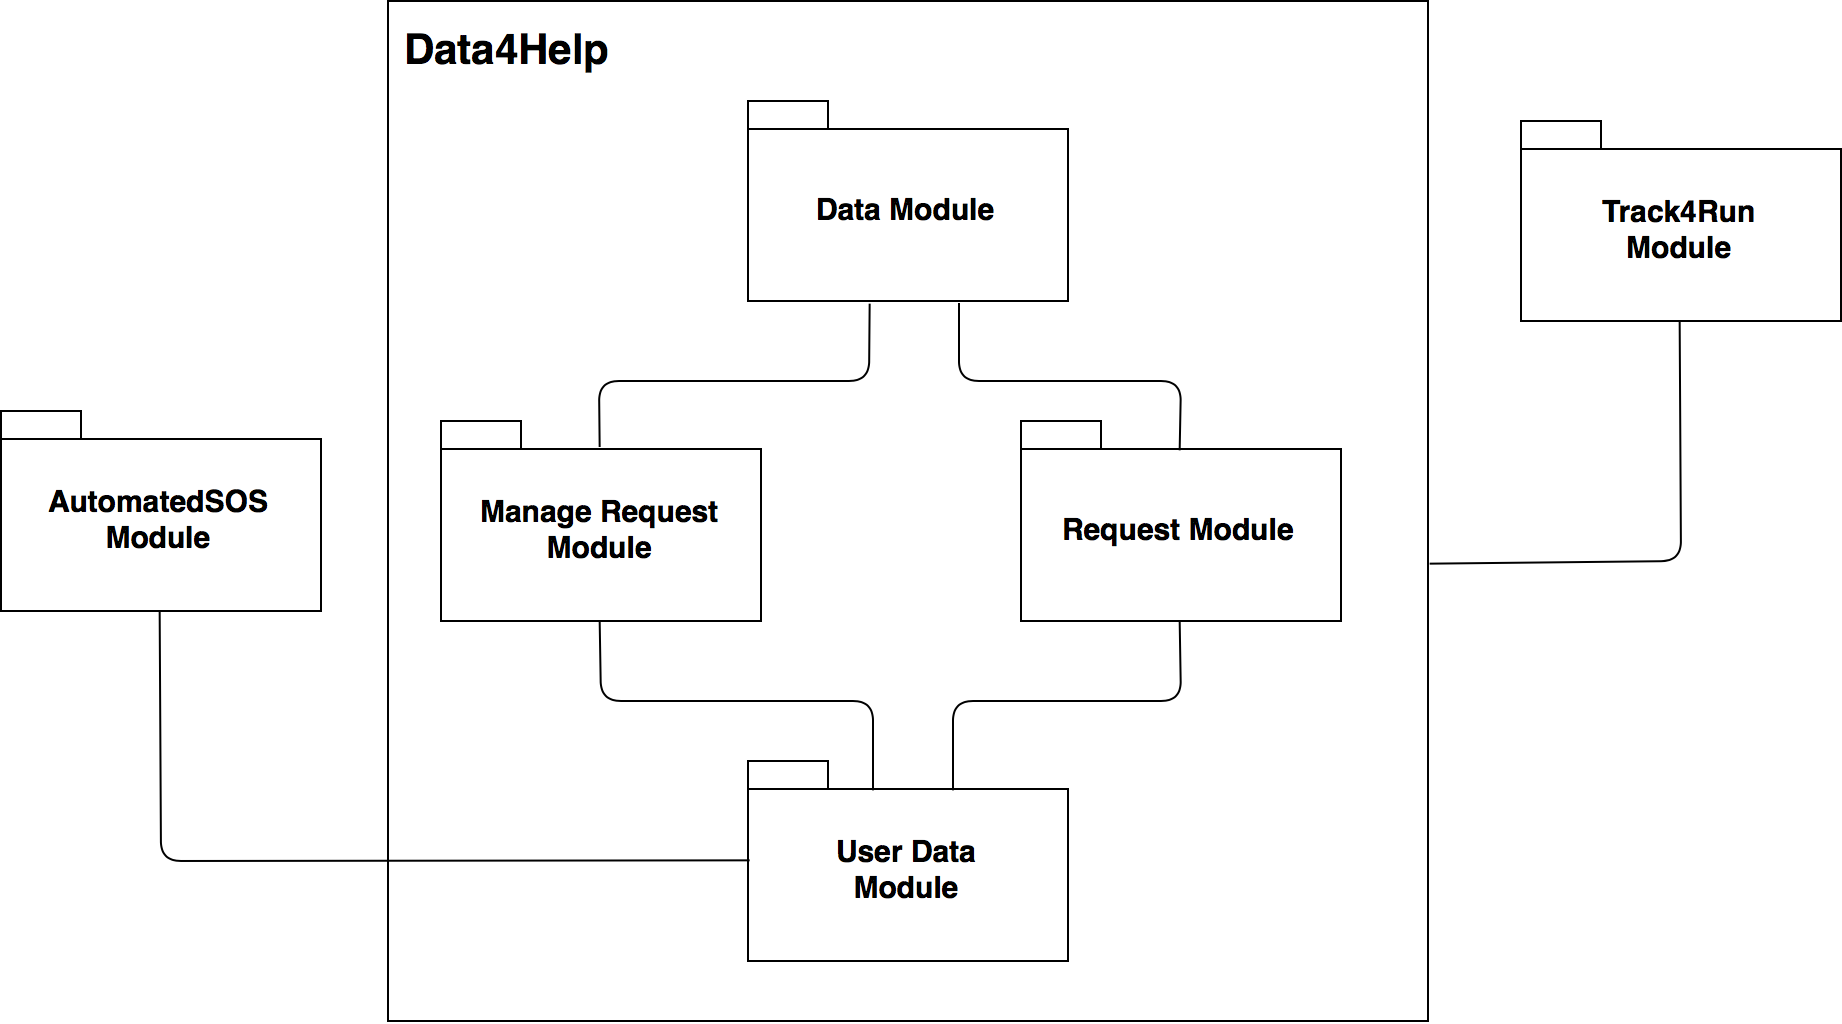
\includegraphics[scale=0.1,keepaspectratio]{DD/Pictures/integration.png}
\centering
\caption{Integration plan}
\end{figure}
 
For example, after completing the manage request module and the request module, the integration between these modules must be done by testing their interaction, i.e. simulating the dispatch and the reply to the requests by the users. 
At the end, load testing and stress testing will be performed on the entire System.

